\documentclass{beamer}
\usetheme{Madrid}
\usepackage[spanish]{babel}
\usepackage{ragged2e}  
\usepackage{multicol}
\setbeamertemplate{caption}[numbered]



% Paquete para posicionar el logo
\usepackage[absolute,overlay]{textpos} 

% Paquete para importar imágenes
\usepackage{graphicx}  

\setbeamertemplate{frametitle}{
  \begin{beamercolorbox}[sep=0.3cm,center,wd=\paperwidth]{frametitle}
    \usebeamerfont{frametitle}\parbox[c][0.8cm][c]{.8\textwidth}{\insertframetitle}\hfill
    \raisebox{-0.3\height}{
\includegraphics[height=0.8cm]{Logos/MarcaBlanco.png}}
  \end{beamercolorbox}
}


\def\supervisor{Dr. Carlos Fuhrhop}
\def\course{Control Avanzado}

\title{ANÁLISIS DE LAZOS DE CONTROL SISO}
\author{Rodrigo Salazar, Elvin Soto}
\institute{UACH}
\date{\today}

% Modificación de la planilla del titulo
\setbeamertemplate{title page}{
  \vbox{}
  \vfill
  \begin{centering}
    %Para llamar a los diferentes logotipos del titulo
    
\includegraphics[height=1.1cm]{Logos/electronica-color.png} \hspace{0.8cm}  
    
\includegraphics[height=1.5cm]{Logos/UACh_Marcacolor.png} \hspace{0.5cm} 
    
\includegraphics[height=0.9cm]{Logos/MarcaColor.png}  
    \par
    \vskip1.5em%
    {\usebeamercolor[fg]{titlegraphic}\inserttitlegraphic\par}
    \begin{beamercolorbox}[sep=8pt,center,colsep=-4bp,rounded=true,shadow=true]{title}
      \usebeamerfont{title}\inserttitle\par%
      \ifx\insertsubtitle\@empty%
      \else%
        \vskip0.25em%
        {\usebeamerfont{subtitle}\usebeamercolor[fg]{subtitle}\insertsubtitle\par}%
      \fi%     
    \end{beamercolorbox}%
    \vskip1em\par
    \begin{beamercolorbox}[sep=8pt,center,colsep=-4bp,rounded=true,shadow=true]{author}
      \usebeamerfont{author}\insertauthor
    \end{beamercolorbox}
    \begin{beamercolorbox}[sep=8pt,center,colsep=-4bp,rounded=true,shadow=true]{author}
      \usebeamerfont{author}Profesor: \supervisor
    \end{beamercolorbox}
    \begin{beamercolorbox}[sep=8pt,center,colsep=-4bp,rounded=true,shadow=true]{author}
        \usebeamerfont{author}Curso: \course
    \end{beamercolorbox}
    \begin{beamercolorbox}[sep=8pt,center,colsep=-4bp,rounded=true,shadow=true]{institute}
      \usebeamerfont{institute}\insertinstitute
    \end{beamercolorbox}
    \begin{beamercolorbox}[sep=8pt,center,colsep=-4bp,rounded=true,shadow=true]{date}
      \usebeamerfont{date}\insertdate
    \end{beamercolorbox}\vskip0.5em
    {\usebeamercolor[fg]{titlegraphic}\inserttitlegraphic\par}
    \par
    \vfill
  \end{centering}
}

\begin{document}
\begin{frame}
  \titlepage
\end{frame}


\begin{frame}
  \frametitle{Contenidos}
  \tableofcontents
\end{frame}


\section{Introducción: Vista Previa}
\begin{frame}{Introducción: Vista Previa}

% El \begin{justify} para dejar el texto en Justificado.
\begin{justify}  
 En el diseño de control se hacen uso de dos técnicas, el análisis y la sintesis:

\vspace{0.3 cm}
\begin{itemize}
     

    \item El \textbf{análisis} se ocupa del impacto que un controlador tiene en un sistema dado cuando interactúan en retroalimentación, 

    \item La \textbf{síntesis} pregunta como construir controladores con ciertas propiedades.

\end{itemize}

 \vspace{0.3 cm}
 Para un controlador y una planta determinados conectados en realimentación, es necesario preguntarse lo siguiente:

\begin{itemize}
 
 \vspace{0.3 cm}
    \item\textbf{¿Es estable el Bucle?} 

 \vspace{0.1 cm}
    \item\textbf{¿Cuales son las sensibilidades a diversas perturbaciones?} 

 \vspace{0.1 cm}
    \item\textbf{¿Como impactan las pequeñas no linealidades en el bucle?} 

\end{itemize}
\end{justify}
\end{frame}


\begin{frame}{Estructuras de retroalimentación}
\begin{justify}

En la figura \ref{lazo cerrado} usaremos las funciones de transferencia y las transformadas de Laplace para describir las relaciones entre el bucle. 

\begin{figure}[H]
    \centering
    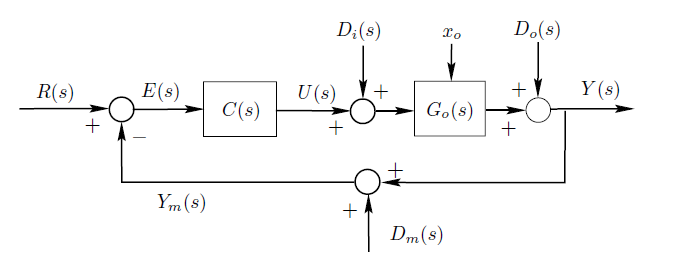
\includegraphics[width=3in]{imagenes/sistema de control retroalimentado simple.PNG}
    \caption{Sistema de control retroalimentado simple}
    \label{lazo cerrado}
\end{figure}


\end{justify}
\end{frame}

\section{Estructuras de retroalimentación}
\begin{frame}{Estructuras de retroalimentación}
\begin{justify}
\footnotesize
\
En particular, $C(s)$ y $G_o(s)$ denotan las funciones de transferencia y el modelo de la planta nominal respectivamente, las cuales pueden ser representadas de forma fraccional de la siguiente forma:

\[C(s)=\frac{P(s)}{L(s)}\]

\[G_o(s)=\frac{B_o(s)}{A_o(s)}\]

\vspace{0.3cm}
$P(s)$, $L(s)$, $B_o(s)$ y $A_o(s)$ son polinomios en el dominio de $s$. $R(s)$, $U(s)$ e $Y(s)$ denotan las transformadas de Laplace de la referencia, la señal de control y la salida de la planta, respectivamente. $D_i(s)$, $D_o(s)$ y $D_m(s)$ denotan la transformada de Laplace del error de entrada, error de salida y el error de medición. También se denota como $x_o$ las condiciones iniciales del modelo.

\end{justify}
\end{frame}

\begin{frame}{Estructuras de retroalimentación}
\begin{justify}
{\footnotesize
De la figura \ref{lazo cerrado} se tienen las siguientes relaciones.
\begin{equation}
Y(s)=G_o(s)U(s)+D_o(s)+G_o(s)D_i(s)+\frac{f(s,x_o)}{A_o(s)}
\end{equation}

\begin{equation}
U(s)=C(s)R(s)-C(s)Y(s)-C(s)D_m(s)
\end{equation}

\[=C(s)\left ( R(s)-D_m(s)-G_o(s)U(s)-D_o(s)-G_o(s)D_i(s)-\frac{f(s,x_o)}{A_o(s)}\right )\]

Donde $f(s,x_o)$ es una función lineal del estado inicial. Las ecuaciones anteriores pueden ser resueltas para dar:

\[U(s)=\frac{C(s)}{1+G_o(s)C(s)} \left ( R(s)-D_m(s)-D_o(s)-G_o(s)D_i(s)-\frac{f(s,x_o)}{A(s)} \right ) \]

\begin{equation*}
    Y(s)= \frac{1}{1+G_o(s)C(s)} \Bigl[ G_o(s)C(s)[R(s)-D_m(s)]  +D_o(s)+G_o(s)D_i(s)+ \frac{f(s,x_o)}{A(s)} \Bigr]
\end{equation*}

}

\end{justify}
\end{frame}


\begin{frame}{Estructuras de retroalimentación}
\begin{justify}
\small

Por lo tanto, si la función de transferencia del controlador C(s) está diseñada para dar una respuesta de señal de referencia particular; es decir.

\vspace{0.3cm}
\[\frac{Y(s)}{R(s)}=\frac{G_o(s)C(s)}{1+G_o(s)C(s)}\]

\vspace{0.3cm}
Entonces esto induce a una respuesta única a la perturbación de salida.

\vspace{0.3cm}
\[\frac{Y(s)}{D_o(s)}=\frac{1}{1+G_o(s)C(s)}\]

\vspace{0.3cm}
Sin embargo, con frecuencia es deseable poder moldear las respuestas de referencia y de perturbación por separado. 

\end{justify}
\end{frame}


\begin{frame}{Estructuras de retroalimentación}
\begin{justify}

{\footnotesize
Esto puede lograrse con la arquitectura de \textit{dos grados de libertad} que se ve en la figura \ref{2 grados de libertad}. 

\vspace{-0.3cm}
\begin{figure}[H]
    \centering
    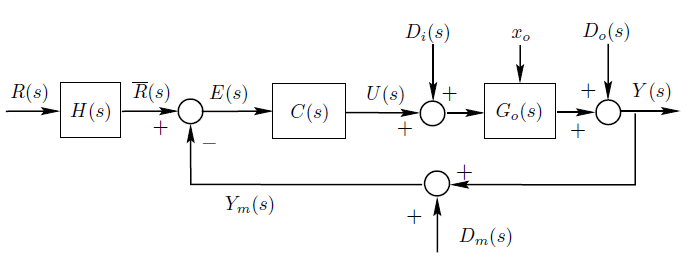
\includegraphics[width=3in]{imagenes/lazo cerrado con 2 grados de libertad.PNG}
    \caption{Lazo cerrado con 2 grados de libertad}
    \label{2 grados de libertad}
\end{figure}
}

\vspace{-0.3cm}
{\tiny

\begin{align*}
Y(s)=& \frac{G_o(s)C(s)H(s)}{1+G_o(s)C(s)}R(s) - \frac{1}{1+G_o(s)C(s)}\Bigl(D_o(s)+\frac{f(s,x_o)}{A_o(s)} \Bigr)
 -\frac{G_o(s)}{1+G_o(s)C(s)}D_i(s)-\frac{G_o(s)C(s)}{1+G_o(s)C(s)}D_m(s)
\end{align*}

\begin{align*}
U(s)=& \frac{C(s)H(s)}{1+G_o(s)C(s)}R(s) - \frac{C(s)}{1+G_o(s)C(s)}\Bigl( D_o(s)+\frac{f(s,x_o)}{A_o(s)} \Bigr)
 -\frac{G_o(s)C(s)}{1+G_o(s)C(s)}D_i(s)-\frac{C(s)}{1+G_o(s)C(s)}D_m(s)
\end{align*}

}

\end{justify}
\end{frame}

% \Huge, \huge, \LARGE, \Large, \large, \normalsize, \small, \footnotesize, \scriptsize, \tiny

\begin{frame}{Estructuras de retroalimentación}
\begin{justify}
\small

La función de transferencia $C(s)$ puede ser diseñada para dar forma a la respuesta de la perturbación y $H(s)$ puede ser usada para dar forma a la respuesta de referencia de forma independiente, donde

\vspace{0.3cm}
\[\frac{Y(s)}{R(s)}=\frac{G_o(s)C(s)H(s)}{1+G_o(s)C(s)}\]

\vspace{0.3cm}
Nótese, sin embargo, que incluso en un bucle de control de dos grados de libertad quedan funciones de transferencia cuya dinámica no se puede configurar de forma independiente.

\vspace{0.3cm}
Por lo tanto, el controlador $C $puede usarse para dar forma a la respuesta a una de las perturbaciones $D_i$, $D_o$ o $D_m$, pero una vez que esto se ha logrado, se determinan las restantes.
\end{justify}
\end{frame}


\begin{frame}{Funciones de sensibilidad nominal}
\begin{justify}
\small

La respuesta del lazo esta gobernada por cuatro funciones de transferencia, conocidas como funciones de sensibilidad, se definen a continuación:

{\footnotesize
\begin{equation} \label{sensibilidad1}
    T_o (s) \stackrel{\Delta}{=} \frac{G_o(s)C(s)}{1+G_o(s)C(s)} = \frac{B_o(s)P(s)}{A_o(s)L(s) + B_o(s)P(s)}
\end{equation}

\begin{equation}\label{sensibilidad2}
    S_o (s) \stackrel{\Delta}{=} \frac{1}{1+G_o(s)C(s)} = \frac{A_o(s)L(s)}{A_o(s)L(s) + B_o(s)P(s)}
\end{equation}

\begin{equation}\label{sensibilidad3}
    S_{io} (s) \stackrel{\Delta}{=} \frac{G_o(s)}{1+G_o(s)C(s)} = \frac{B_o(s)L(s)}{A_o(s)L(s) + B_o(s)P(s)}
\end{equation}

\begin{equation}\label{sensibilidad4}
    S_{uo} (s) \stackrel{\Delta}{=} \frac{C(s)}{1+G_o(s)C(s)} = \frac{A_o(s)P(s)}{A_o(s)L(s) + B_o(s)P(s)}
\end{equation}

\begin{align*}
    S_o (s) + T_o(s) &= 1, & S_{io} (s) &= S_o(s)C(s) = \frac{T_o(s)}{C(s)}, & S_{uo} (s) &= S_o(s)C(s) = \frac{T_o(s)}{G_o(s)}
\end{align*}

}
\end{justify}
\end{frame}


\begin{frame}{Funciones de sensibilidad nominal}
\justifying
{\small
\vspace{0.1 cm}
Las ecuaciones de sensibilidad anteriormente decritas, se puede expresar de forma mas compacta como:
\vspace{0.1 cm}

% \Huge, \huge, \LARGE, \Large, \large, \normalsize, \small, \footnotesize, \scriptsize, \tiny
}
{\footnotesize
\begin{equation}\label{ecuacioncompacta} %nombre para referenciarla
\begin{bmatrix}
Y_o(s) \\
U_o(s)
\end{bmatrix}
=
\frac{\begin{bmatrix}
G_o(s)C_o(s) & G_o(s) & 1 & -G_o(s)C(s) \\
C(s) & -G_O(s)C(S) & -C(s) & -C(s) 
\end{bmatrix}}{1 + G_o(s)C(s)}
\begin{bmatrix}
H(s)R(S) \\
D_i(s) \\
D_o(s) \\
D_m(s)
\end{bmatrix}
\end{equation}
}
\end{frame}

\begin{frame}{Funciones de sensibilidad nominal}
\begin{justify}
\textbf{Ejemplo:}

\vspace{0.3cm}
Una planta modelada nominalmente por $G_o(s) = \frac{4}{(s+1)(s+2)^2}$. La planta tiene una perturbación de salida dada por $d_o(t) = k + d_v(t)$ donde $d_v(t)$  es una señal de media cero con energía en la banda $B_d: (0,4)[rad/s]$.
Un controlador de retroalimentación $C(s)$ está diseñado para que

\vspace{0.3 cm}
\begin{equation}
    T_o(s) = \frac{\alpha}{(s^2+1.2\omega_ns + \omega_n^2)(\tau s + 1)^2}
\end{equation}

\vspace{0.3 cm}
El factor $(\tau s + 1)$ se selecciona para que el controlador sea adecuado. Se pide discutir la elección de $\alpha$ y $\omega_n$ desde el punto de vista de compensación de perturbaciones de salida y la magnitud del esfuerzo de control requerido.

\end{justify}
\end{frame}


\begin{frame}{Funciones de sensibilidad nominal}
\begin{justify}
\textbf{Solución:}

\vspace{0.3 cm}
Necesitamos $T_o(j\omega)\approx 1$ (Lo que implica $S_o(j\omega)\approx 0$) en $\omega = 0$ y en $B_d$. Para lograr esto:

\vspace{0.3 cm}
\begin{itemize}
    \item $\alpha = \omega_n^2$
    \item $\omega_n$ mayor a $4[rad/s]$.  Digamos $\omega_n = 10[rad/s]$
    \item $\tau = 0.01$ (que es mucho menor que $\omega_n^{-1}$)
\end{itemize}

\vspace{0.3 cm}
Esto lleva a:

\vspace{0.3 cm}
\begin{equation}
    T_o(s) = \frac{100}{(s^2 + 12s + 100)(0.01s + 1)}
\end{equation}

\end{justify}
\end{frame}


\begin{frame}{Funciones de sensibilidad nominal}
\begin{justify}

Luego verificamos la sensibilidad de control nominal $S_{uo}(s)$. Para la elección anterior de $T_o$, tenemos

\vspace{0.3 cm}
{\small
\begin{equation*}
    S_{uo}(s) = \frac{T_o(s)}{G_o(s)} = 25\frac{(s+1)(s+2)^{2}}{(s^2 + 12s + 100)(0.01s + 1)^{2}}
\end{equation*}
}

\vspace{0.3 cm}
A ${3}[rad/s]$ tenemos que $|S_{uo}(j\omega)| \approx {20}[dB]$. Esto significa que si $d_v(t)$ tiene una componente sinusoidal a ${3}[rad/s]$, entonces la salida del controlador tendría una componente de la misma frecuencia con una amplitud diez veces mayor que la de la perturbación.
Esto podría conducir a la saturación de la entrada. Reflexionando, podemos ver que este
problema surge porque la perturbación de salida tiene un ancho de banda que es mucho
mayor que el de la planta de bucle abierto.

\end{justify}
\end{frame}


\begin{frame}{Estabilidad en bucle cerrado basada en el polinomio característico}
\begin{justify}
\textit{Se dice que el bucle nominal es internamente estable si y solo si todas las 8 funciones de transferencia en la ecuación \ref{ecuacioncompacta} son estables }. 

\vspace{0.3cm}
La definición anterior es exigir que todas las señales del ciclo estén limitadas para cada conjunto de entradas limitadas $r(t), d_i(t), d_o(t) y d_m(t)$. Las ecuaciones en \ref{ecuacioncompacta} muestran que el lazo nominal cerrado es internamente estable si y solo si el polinomio $A_o(s)L(s)+B_o(s)P(s)$ tiene factores estables. Por lo tanto, decimos que un sistema es internamente estable si y solo si las raices de la ecuación caracteristica del lazo cerrado nominal se encuentran en el semi plano izquierdo abierto.

\begin{equation}\label{ecua-caracteristica}
    A_o(s)L(s)+B_o(s)P(s)=0
\end{equation}


\end{justify}
\end{frame}

\section{Estabilidad en bucle cerrado basada en el polinomio característico}
\begin{frame}{Estabilidad en bucle cerrado basada en el polinomio característico: Ejemplo 2}
\begin{justify}
Supongamos que

\[G_o(s)=\frac{3}{(s+4)(-s+2)} \qquad C(s)=\frac{-s+2}{s}\]

\vspace{0.3cm}
Puede verse que $T_o(s)$ es estable. Sin embargo la sensibilidad de perturbación de entrada nominal es inestable ya que

\[S_{io}(s)=\frac{3s}{(-s+2)(s^2+4s+3)}\]

\vspace{0.3cm}
Por lo tanto, el sistema no es internamente estable y no satisface la definición dicha anteriormente, dado que $A_o(s)L(s)+B_o(s)P(s)=(-s+2)(s^2+4s+3)$.

\end{justify}
\end{frame}


\section{Análisis de Estabilidad y Polinomios}
\begin{frame}{Análisis de Estabilidad y Polinomios}
\begin{justify}
\textbf{Definición del Problema}
\vspace{0.3cm}

Considere el polinomio $p(s)$ definido por
\[p(s)=s^n+a_{n-1}s^{n-1}+ ... +a_1s+a_o\]



El problema a estudiar trata sobre si ese polinomio tiene alguna raíz con parte real no negativa. Obviamente, esta pregunta puede responderse calculando las $n$ raíces de $p(s)$. Sin embargo, en muchas aplicaciones, es de especial interés estudiar la interacción entre la ubicación de las raíces y ciertos coeficientes polinómicos. Los polinomios que tienen todas sus raíces en el plano izquierdo cerrado (es decir, con partes reales no positivas) se conocen como polinomios de Hurwitz. Si restringimos las raíces para que tengan partes reales negativas, decimos que el polinomio es estrictamente de Hurwitz.

\end{justify}
\end{frame}



\begin{frame}{Análisis de Estabilidad y Polinomios: Algoritmo de Routh}
\begin{justify}

% \Huge, \huge, \LARGE, \Large, \large, \normalsize, \small, \footnotesize, \scriptsize, \tiny
{\footnotesize
Uno de los algoritmos más populares para determinar si un polinomio es o no estrictamente de Hurwitz es el algoritmo de Routh. El algoritmo se basa en la siguiente matriz numérica:



\begin{table}[t]
   

\begin{center}
\begin{tabular}{c|ccccc}
$s^n$ & $\gamma_{0,1}$ & $\gamma_{0,2}$ & $\gamma_{0,3}$ & $\gamma_{0,4}$ & ...\\ 
$s^{n-1}$ & $\gamma_{1,1}$ & $\gamma_{1,2}$ & $\gamma_{1,3}$ & $\gamma_{1,4}$ & ... \\
$s^{n-2}$ & $\gamma_{2,1}$ & $\gamma_{2,2}$ & $\gamma_{2,3}$ & $\gamma_{2,4}$ & ...\\
$s^{n-3}$ & $\gamma_{3,1}$ & $\gamma_{3,2}$ & $\gamma_{3,3}$ & $\gamma_{3,4}$ & ...\\
$s^{n-4}$ & $\gamma_{4,1}$ & $\gamma_{4,2}$ & $\gamma_{4,3}$ & $\gamma_{4,4}$ & ...\\
$\vdots$ & $\vdots$ & $\vdots$ & $\vdots$ & $\vdots$\\
$s^{2}$ & $\gamma_{n-2,1}$ & $\gamma_{n-2,2}$\\
$s^{1}$ & $\gamma_{n-1,1}$ \\
$s^{0}$ & $\gamma_{n,1}$
\end{tabular}
\caption{Matriz de Routh}
\label{matriz Routh}

\end{center}
\end{table}

 Donde $\gamma_{k,j}$ se puede calcular como

\begin{equation}
\gamma_{k,j} = \frac{\gamma_{k-1,1} \gamma_{k-2,j+1} - \gamma_{k-2,1} \gamma_{k-1,j+1}}{\gamma_{k-1,1}}, \quad k = 2, \dots, n, \quad j = 1, 2, \dots, m_j
\end{equation}
}
 
\end{justify}
\end{frame}

\begin{frame}{Análisis de Estabilidad y Polinomios: Algoritmo de Routh}
\begin{justify}
\textbf{Ejemplo} Consideremos \( p(s) = s^5 + 5s^4 + 12s^3 + 13s^2 + 3s + 6 \). Primero observamos que todos los coeficientes de este polinomio son mayores que cero, por lo que no podemos descartar que este polinomio sea un polinomio de Hurwitz. Para verificarlo, construimos el arreglo de Routh:

{\footnotesize
\begin{center}
\begin{tabular}{c|ccccc}
$s^5$ & $1$ & $12$ & $3$ &  &  \\ 
$s^4$ & $5$ & $13$ & $6$ &  &  \\
$s^3$ & $\frac{47}{5}$ & $\frac{9}{5}$ &  &  &  \\
$s^2$ & $\frac{566}{47}$ & $6$ &  &  &  \\
$s^1$ & $-\frac{8160}{235}$ &  &  &  &  \\
$s^0$ & $6$ &  &  &  &  \\
\end{tabular}
\label{matriz Routh}
\end{center}
}

De este arreglo observamos que hay dos cambios de signo en la primera columna. De acuerdo con el criterio de Routh, esto significa que \( p(s) \) tiene dos raíces con partes reales positivas. Por lo tanto, \( p(s) \) no es un polinomio de Hurwitz.

\end{justify}
\end{frame}

\begin{frame}{Análisis de Estabilidad y Polinomios: Algoritmo de Routh}
\begin{justify}

  Entonces, el número de raíces con parte real mayor que cero es igual al número de cambios de signo en la primera columna de la matriz.

 \vspace{0.3cm}
 Al usar la matriz de Routh, a veces hay casos especiales que requieren que se tomen medidas adicionales. Por ejemplo, vemos que al construir la matriz, no podemos continuar cuando uno de los elementos en la primera columna es cero. Esto se puede tratar de la siguiente forma.


\end{justify}
\end{frame}

\begin{frame}{Análisis de Estabilidad y Polinomios: Algoritmo de Routh: Caso 1}
\begin{justify}

 Primero consideramos el caso cuando el primer elemento en la columna asociado con $S^{n-k}$ es cero pero hay al menos otro elemento distinto de cero.\\

 En este caso sustituimos el termino $\gamma_{k,1}$ por un $\epsilon$, donde $\epsilon$ es un numero de una magnitud muy pequeña, con el mismo signo que el de $\gamma_{k-1,1}$, es decir, se utiliza $\left | \epsilon \right |$ o $-\left | \epsilon \right |$. Entonces la matriz es completada y se aplica el criterio de Routh para saber si el polinomio es o no estrictamente de Hurwitz, pues $\left | \epsilon \right | \rightarrow 0^+$ 


\end{justify}
\end{frame}

\begin{frame}{Análisis de Estabilidad y Polinomios: Algoritmo de Routh: Caso 1}
\begin{justify}

 Como ejemplo consideramos el polinomio $p(s)=s^5+3s^4+2s^3+6s^2+3s+3$. Entonces tenemos que el arreglo de Routh es
\[
\begin{tabular}{c|ccccc}
$s^5$ & 1 & 2 & 3 \\ 
$s^4$ & 3 & 6 & 3 \\
$s^3$ & 0 & 2 \\
$s^2$ \\
$s^1$ \\
$s^0$ 

\end{tabular}
\qquad
\Rightarrow 
\quad
\begin{tabular}{c|ccccc}
$s^5$ & 1 & 2 & 3 \\ 
$s^4$ & 3 & 6 & 3 \\
$s^3$ & $\left | \epsilon \right |$ & 2 \\
$s^2$ & 6-$\frac{6}{\left | \epsilon \right |}$ & 3\\
$s^1$ & 2+$\frac{\left | \epsilon \right |^2}{1-2\left | \epsilon \right |}$  \\
$s^0$ & 3
\end{tabular}
\]
Entonces observamos que al hacer $\left | \epsilon \right | \rightarrow 0^+$  hay dos cambios de signo,es decir p(s) no es Hurwitz ya que tiene dos raíces con partes reales positivas.

\end{justify}
\end{frame}

\begin{frame}{Análisis de Estabilidad y Polinomios: Algoritmo de Routh: Caso 2}
\begin{justify}
A continuación, consideramos el caso en el que todos los elementos de la fila con $s^{n-k}$ son ceros, es decir $\gamma_{k,1} = \gamma_{k,2} ... = 0$.

En este caso, el polinomio original puede ser factorizado por el polinomio $p_a(s)=\gamma_{k-1,1}s^{n-k+1} + \gamma_{k-1,2}s^{n-k-1} + \gamma_{k-1,3}s^{n-k-3} + ... $ tenga en cuenta que este es solo un polinomio de potencias pares o impares de $s$ donde los coeficientes corresponden a los términos en la fila justo arriba de la fila cero. 

\end{justify}
\end{frame}



\begin{frame}{Análisis de Estabilidad y Polinomios: Algoritmo de Routh: Caso 2}
\begin{justify}

\subsection*{Ejemplo 5.6}
Considere el polinomio $p(s) = s^6 + 5s^5 + 2s^4 + 5s^3 + 4s^2 + 15s + 3$, el arreglo de Routh asociado es

% Insert the Routh table using the format provided
{\footnotesize
\begin{center}
\begin{tabular}{c|ccccc}
$s^6$ & $1$ & $2$ & $4$ & $3$ \\ 
$s^5$ & $5$ & $5$ & $15$ &  \\ 
$s^4$ & $1$ & $1$ & $3$ &  \\ 
$s^3$ & $0$ & $0$ &  &  \\ 
$s^2$ &  &  &  &  \\ 
$s^1$ &  &  &  &  \\ 
$s^0$ &  &  &  &  \\ 
\end{tabular}
\end{center}
}

Así, $p_a(s) = s^4 + s^2 + 3$. Luego, por división polinómica, obtenemos $p(s) = p_a(s)(s^2 + 5s + 1)$. Note que las raíces de $p_a(s)$ están localizadas en $\pm 0.7849 \pm j1.0564$.

\end{justify}
\end{frame}


\begin{frame}{Análisis de Estabilidad y Polinomios: Algoritmo de Routh: Caso 2}
\begin{justify}
\footnotesize
El algoritmo de Routh se puede aplicar al denominador de una función de transferencia para determinar si el sistema es estable o no. Sin embargo, también puede ser utilizado para estudiar los efectos de la variación de parámetros en la estabilidad del sistema. 

\vspace{0.2cm}
\textbf{Ejemplo:}

\vspace{0.2cm}
Calculamos el polinomio característico de lazo cerrado, que viene dado por $p(s) = s^3 + 2s^2 + s + K$, y luego construimos el arreglo de Routh


\begin{table}[t]
\begin{center}
\begin{tabular}{c|ccccc}
$s^3$ & 1 & 1 && \\
$s^2$ & 2 & K && \\
$s^1$ & $1 -0.5K$ & & & \\
$s^0$ & K & & & \\
\end{tabular}
\label{matriz Routh}
\end{center}
\end{table}


\vspace{0.1cm}
Ahora podemos ver que no hay polos inestables en lazo cerrado si y solo si $1 - 0.5K > 0$ y $K > 0$. Combinando estos dos requisitos, tenemos que el lazo cerrado es estable si y solo si $0 < K < 2$. Ahora podemos ver que no hay polos inestables en lazo cerrado si y solo si $1 - 0.5K > 0$ y $K > 0$. Combinando estos dos requisitos, tenemos que el lazo cerrado es estable si y solo si $0 < K < 2$.



\end{justify}
\end{frame}


\subsection{Root Locus}
\begin{frame}{Análisis de Estabilidad y Polinomios: Lugar geométrico de las raíces (Root Locus)}
\begin{justify}

Otra herramienta clásica utilizada para estudiar la estabilidad de ecuaciones del tipo dado en la ecuación \ref{ecua-caracteristica} es el lugar geométrico de las raíces. 

\vspace{0.3 cm}
El enfoque del lugar geométrico de las raíces se puede utilizar para examinar la ubicación de las raíces del polinomio característico cuando se varía un parámetro (generalmente el parámetro K del controlador). 

\vspace{0.3 cm}
Por ejemplo, suponga que el modelo de planta nominal viene dado por $G_o(s)$ y que el controlador tiene una función de transferencia descrita como $C(s) = KC_a(s)$, donde $C_a(s)$ es un cociente conocido de dos polinomios mónicos en $s$ y $K$ es una constante positiva, pero desconocida. Entonces, los polos en lazo cerrado son las raíces de

\begin{equation}\label{ecua-caracteristica-1}
    1 + KC_a(s)G_o(s) = 0
\end{equation}

\end{justify}
\end{frame}

\begin{frame}{Análisis de Estabilidad y Polinomios: Lugar geométrico de las raíces (Root Locus)}
\begin{justify}

El conjunto de todos los puntos en el plano complejo que satisfacen la ecuacion \ref{ecua-caracteristica-1} para algún valor positivo de $K$ se conoce como lugar geométrico de las raíces. Este problema particular puede integrarse en el siguiente problema más general. Considere la siguiente ecuación:

\begin{equation}\label{ecua-caracteristica-p1}
    1 + \lambda F(s) = 0, \ \ \ \text{ donde } \ \ \ F(s)= \frac{M(s)}{D(s)}
\end{equation}

con $\lambda \geq 0$ y

{\footnotesize
\begin{equation*}\label{polinomio-m}
    M(s) = s^{m} + b_{m-1}s^{m-1}+ ... + b_1s + b_0 = \prod_{i=1}^{m} (s-c_i)
\end{equation*}
}
{\footnotesize
\begin{equation*}\label{polinomio-m}
    D(s) = s^{n} + b_{n-1}s^{n-1}+ ... + b_1s + b_0 = \prod_{i=1}^{n} (s-p_i)
\end{equation*}
}

\end{justify}
\end{frame}




\begin{frame}{Análisis de Estabilidad y Polinomios: Lugar geométrico de las raíces (Root Locus)}
\begin{justify}
Observamos que la solución de la ecuación \ref{ecua-caracteristica-1} es también la solución de la ecuación:

{\footnotesize
\begin{equation}\label{polinomio-m2}
    D(s) + \lambda M(s) = \prod_{i=1}^{n} (s-p_i) + \lambda\prod_{i=1}^{m} (s-c_i)
\end{equation}
}

\vspace{0.3cm}
Las reglas de construcción del lugar de las raíces incluyen:

\vspace{0.2cm}
\begin{itemize}
    \item \textbf {R1:} El número de raíces en la ecuación \ref{polinomio-m2} es igual a max (m, n). Por lo tanto, el lugar geométrico de las raíces tiene un máximo de (m, n) ramas.

    \vspace{0.3cm}
    \item \textbf {R2:} De la ecuación \ref{ecua-caracteristica-1} observamos que $s_0$ pertenece al lugar geométrico de las raíces (para $\lambda \geq 0$) si y solo si

    {\footnotesize
    \begin{equation}\label{regla-2}
        argF(s_0) = (2k+1)\pi
    \end{equation}
    }

    
\end{itemize}

\end{justify}
\end{frame}


\begin{frame}{Análisis de Estabilidad y Polinomios: Lugar geométrico de las raíces (Root Locus)}
\begin{justify}

\begin{itemize}
    \justifying
    \item \textbf{R3:} De la ecuación \ref{ecua-caracteristica-1}  observamos que si $s_0$ pertenece al lugar geométrico de las raíces, el valor correspondiente de $\lambda$ es $\lambda_0$, donde

    {\footnotesize
    \begin{equation}\label{lambda-cero}
        \lambda_0 = \frac{-1}{F(s_0)}
    \end{equation}
    }

    \vspace{0.3cm}
    \item \textbf{R4:} Un punto $s_0$ en el eje real, es decir, $s_0 \in \mathbb{R}$, es parte del lugar geométrico de las raíces (para $\lambda \geq 0$), si y solo si, está ubicado a la izquierda de un número impar de polos y ceros (de modo que \ref{regla-2} se cumple).

    \vspace{0.3cm}
    \item \textbf{R5:} Cuando $\lambda$ es cercano a cero, entonces $n$ de las raíces están ubicadas en los polos de $F(s)$, es decir, en $p_1, p_2,... ,p_n$ y, si $n< m$, las otras ${m} - {n}$ raíces están ubicadas en $ \infty $ .
  
\end{itemize}

\end{justify}
\end{frame}

\begin{frame}{Análisis de Estabilidad y Polinomios: Lugar geométrico de las raíces (Root Locus)}
\begin{justify}

\begin{itemize}

    \justifying
    \item \textbf{R6:} Cuando $\lambda$ está cerca de $\infty$, entonces $m$ de estas raíces se ubican en los ceros de $F(s)$, es decir, en $c_1, c_2,... ,c_m$ y, si $n > m$, las otras $n - m$ raíces se ubican en $\infty$.

    \vspace{0.3cm}
    \item \textbf{R7:} Si $n>m$, y $\lambda$ tiende a $ \infty $, entonces, ${n}-{m}$ raíces tienden asintóticamente a $\infty$, siguiendo asíntotas que se cortan en $(\sigma, 0)$, donde 

    \vspace{0.3cm}
    {\small
    \begin{equation}\label{regla-7}
        \sigma = \frac{\sum_{i=1}^{n} p_i - \sum_{i=1}^{m} c_i}{n-m} 
    \end{equation}
    }

        Los ángulos de estas asíntotas son $\eta_1, \eta_2,...\eta_{n-m}$, donde

    {\small
    \begin{equation}\label{regla-7.1}
        \eta_1 = \frac{(2k-1)\pi}{n-m} ;  \ \ \  \ \ \  k = 1,2,....,n-m
    \end{equation}
    }

\end{itemize}
\end{justify}
\end{frame}

\begin{frame}{Análisis de Estabilidad y Polinomios: Lugar geométrico de las raíces (Root Locus)}
\begin{justify}

\begin{itemize}
    \justifying
    \item \textbf {R8:} Si $n< m$, y $\lambda$ tiende a cero, entonces, ${m} - {n}$ raíces tienden asintóticamente a $ \infty $, siguiendo asíntotas que se cortan en $(\sigma, 0)$, donde
    
    \vspace{0.3cm}
    {\small
    \begin{equation}\label{regla-8}
        \sigma = \frac{\sum_{i=1}^{n} p_i - \sum_{i=1}^{m} c_i}{m-n} 
    \end{equation}
    }
    Los ángulos de estas asíntotas son $\eta_1, \eta_2,...\eta_{m-n}$, donde

    {\small
    \begin{equation}\label{regla-8.1}
        \eta_1 = \frac{(2k-1)\pi}{n-m} ;  \ \ \  \ \ \  k = 1,2,....,m-n
    \end{equation}
    }
    
    \vspace{0.3cm}
    \item \textbf{R9:} Cuando el lugar geométrico de las raíces cruza el eje imaginario, digamos en $s = ±j\omega_c$, entonces $\omega_c$ se puede calcular usando el algoritmo de Routh Hurwitz, o usando el hecho de que $s_2 + \omega_2$ c divide exactamente el polinomio $D(s) + \lambda M(s)$, para algún valor real positivo de $\lambda$.

\end{itemize}

\end{justify}
\end{frame}


\begin{frame}{Análisis de Estabilidad y Polinomios: Lugar geométrico de las raíces (Root Locus)}
\begin{justify}
\textbf{Ejemplo [1]:}

\vspace{0.3cm}
Considere una planta $G_o(s)$ y un controlador de retroalimentación $H(s)$, donde:

{\small
\begin{equation*}\label{rl-ejemplo-1}
    G_o(s) = \frac{1}{s(s+1)(s+2)}  \  \ \ \  \text{ y } \ \ \ \ H(s) = K, (para: K=1)
\end{equation*}
}
1) Determinar los polos y ceros
{\small
\begin{equation*}\label{rl-ejemplo-1}
    s_1=0, s_2=-1, s_3=-2
\end{equation*}
}

2) Obtener el lugar geometrico de las raices (\textbf{R5}) en el eje real  $[0, \infty)$
y 3) Centroide de las asintotas 
{\small
\begin{equation*}\label{rl-ejemplo-1}
    \sigma_c = \frac{\sum polos - \sum ceros}{n-m}, n=3 (polos), m=0 (ceros)
\end{equation*}
}
{\small
\begin{equation*}\label{rl-ejemplo-1}
    \sigma_c = \frac{-2 - 1}{3}=-1
\end{equation*}
}
\end{justify}
\end{frame}

\begin{frame}{Análisis de Estabilidad y Polinomios: Lugar geométrico de las raíces (Root Locus)}
\begin{justify}
\begin{itemize}
4) Determinar las asintotas
{\small
\begin{equation*}\label{rl-ejemplo-1}
    \theta_k = \frac{(2k-1)(180)}{n-m}
\end{equation*}
}
{\small
\begin{equation*}\label{rl-ejemplo-2}
   k=1 \rightarrow \theta_1 = 60^\circ
\end{equation*}
}
{\small
\begin{equation*}\label{rl-ejemplo-2}
   k=2 \rightarrow \theta_2 = 180^\circ
\end{equation*}
}
{\small
\begin{equation*}\label{rl-ejemplo-2}
   k=3 \rightarrow \theta_3 = 300^\circ
\end{equation*}
}
\\
Normalmente encontrará que un ángulo es la reflexión respecto al eje Real del otro ángulo.
\end{itemize}
\end{justify}
\end{frame}


\begin{frame}{Análisis de Estabilidad y Polinomios: Lugar geométrico de las raíces (Root Locus)}
\begin{justify}
\begin{itemize}
 5) Puntos de ruptura o ingreso,
 Se calcula encontrando los máximos y los mínimos de K. Primero se despeja para k, luego se deriva y se iguala a cero para encontrar los máximos y mínimos.
 \begin{equation*}\label{rl-ejemplo-2}
   kG(s)=\frac{k}{s(s+1)(s+2)}=-1
\end{equation*}
\\
Despejando para K y derivando tenemos
\\
 \begin{equation*}\label{rl-ejemplo-2}
   \frac{dk}{ds}=-(3s^2+6s+2)=0
\end{equation*}
 \begin{equation*}\label{rl-ejemplo-2}
   S_{c1}=-0.4226
\end{equation*}
 \begin{equation*}\label{rl-ejemplo-2}
    S_{c2}=-1.5774
\end{equation*}

\end{itemize}
\end{justify}
\end{frame}

\begin{frame}{Análisis de Estabilidad y Polinomios: Lugar geométrico de las raíces (Root Locus)}
\begin{justify}
\begin{itemize}
\justifying
 6) Ganancia crítica
 \begin{equation*}\label{rl-ejemplo-2}
   1+kG(s)=1+\frac{k}{s(s+1)(s+2)}
\end{equation*}
\begin{equation*}\label{rl-ejemplo-2}
  s(s+1)(s+2)+K
\end{equation*}
\\
sustituyendo $s=j\omega$ (evaluarlo en el eje imaginario)
\\
 \begin{equation*}\label{rl-ejemplo-2}
   1+G(j\omega)H(j\omega)=(j\omega)^3+3(j\omega)^2+2(j\omega)+k
\end{equation*}
 \begin{equation*}\label{rl-ejemplo-2}
  (k-3\omega^2)+(2\omega-\omega^3)j=0+0j
\end{equation*}
Igualando la parte real y la parte imaginaria respectivametne y encontrando el valor de $\omega$, encontramos el valor de K,
dando como resultado:
\\
k=0, $\omega$=0,$-\sqrt{2}$, $\sqrt{2}$

\end{itemize}
\end{justify}
\end{frame}

\begin{frame}{Análisis de Estabilidad y Polinomios: Lugar geométrico de las raíces (Root Locus)}
\begin{justify}

\begin{itemize}
    \begin{figure}[H]
    \centering
    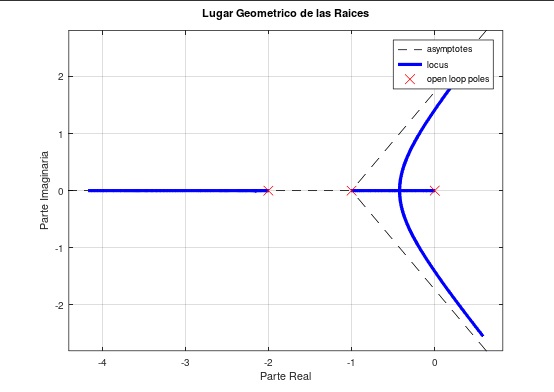
\includegraphics[width=3.5in]{imagenes/LGRResuelto.png}
    \caption{Resultado del ejercicio}
    \label{niquist-function}
    \end{figure}   
\end{itemize}

\end{justify}
\end{frame}

\section{Estabilidad nominal usando la respuesta en frecuencia}
\begin{frame}{Estabilidad nominal usando la respuesta de frecuencia}
\begin{justify}

\begin{itemize}
    \justifying
    Una herramienta clásica para evaluar la estabilidad de un circuito de retroalimentación es la teoría de la estabilidad de Nyquist utilizando la respuesta de frecuencia del sistema en circuito abierto. Esto se logra trazando un diagrama polar del producto Go(s)C(s) y luego contando el número de círculos del punto (-1, 0). 
    Primero consideraremos una función de transferencia arbitraria F(s) (no necesariamente relacionada con el control en bucle cerrado).
    
    \vspace{0.3cm}
    \item La teoría de la estabilidad de Nyquist depende de mapeos entre dos planos complejos: 
    
    \vspace{0.3cm} 
    \item Las variables independientes s
    
    \vspace{0.3cm} 
    \item La variable dependiente F
\end{itemize}

\end{justify}
\end{frame}

\section{Análisis de estabilidad de Nyquist}
\begin{frame}{Análisis de estabilidad de Nyquist}
\begin{justify}

\begin{itemize}
    \justifying
    Esto tiene una conexión directa con la cuestión de la estabilidad del circuito cerrado. Para aplicar este resultado, consideramos una función especial $F(s)$, relacionada con la FT en lazo abierto de la planta, $G_o$, y un controlador $C(s)$ mediante la relación simple:
    \vspace{0.2cm} 
    \item 
    \[F (s) = 1 + G_o(s)C(s)\]
    \vspace{0.2cm} 
    \item 
    Observamos que los ceros de $F(s)$ son los Polos LC en un sistema de control con retroalimentación unitaria y los polos de $F(s)$ son los polos en BA de la planta y el controlador.
    Suponemos que $G_o(s)C(s)$ es estrictamente apropiado de modo que $F(s)$ satisface
    \[\lim_{\left | s \right | \to \infty } F(s)=1\]
\end{itemize}

\end{justify}
\end{frame}

\begin{frame}{Análisis de estabilidad de Nyquist}
\begin{justify}
\begin{itemize}
     \justifying
     Esta curva combina el eje imaginario $C_i$ y la curva de retorno $C_r$ (un semicírculo de radio infinito) como se muestra en la figura. Esta elección de C se conoce como camino de Nyquist.
    \begin{figure}[H]
    \centering
    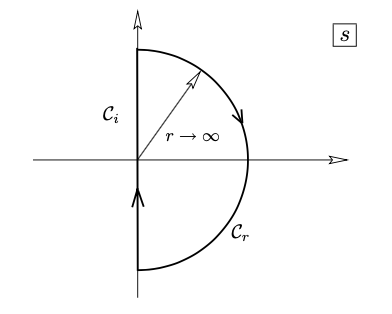
\includegraphics[width=2in]{imagenes/nyquist-path.png}
    \caption{Nyquist path}
    \label{niquist-function}
    \end{figure}
\end{itemize}

\end{justify}
\end{frame}


\begin{frame}{Análisis de estabilidad de Nyquist}
\begin{justify}

\begin{itemize}
\justifying
    \item Si el sistema es estable en lazo abierto, entonces para que el lazo cerrado sea internamente estable es necesario y suficiente que no ocurran cancelaciones inestables y que la gráfica de Nyquist de $G_o(s)C(s)$ no rodee el punto $(-1, 0)$
    \vspace{0.3cm}
    \item Si el sistema es inestable en bucle abierto, con polos P en el RHP abierto, entonces para que el bucle cerrado sea internamente estable es necesario y suficiente que no se produzcan cancelaciones inestables y que la gráfica de Nyquist de $G_o(s)C(s)$ rodee el punto $(-1, 0)$ P veces en sentido antihorario
    \vspace{0.3cm}
    \item Si el diagrama de Nyquist de $G_o(s)C(s)$ pasa exactamente por el punto $(-1, 0)$, existe un $\omega_o$ que pertenece a R tal que $F(j\omega_o) = 0$, es decir, el circuito cerrado tiene polos ubicados exactamente en el eje imaginario.
    
\end{itemize}

\end{justify}
\end{frame}

\begin{frame}{Análisis de estabilidad de Nyquist}
\begin{justify}

\begin{itemize}

   Queda pendiente una cuestión importante: cómo aplicar la teoría de Nyquist cuando hay polos en bucle abierto exactamente en el eje imaginario.
    \begin{figure}[H]
    \centering
    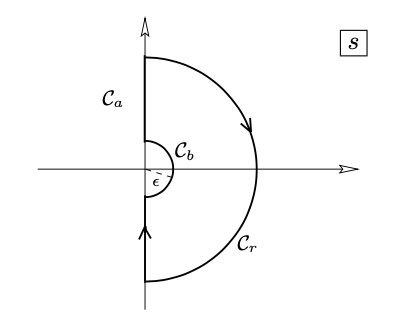
\includegraphics[width=2in]{imagenes/nyquist-modificado.png}
    \caption{Nyquist path con un polo en el eje imaginario}
    \label{niquist-function}
    \end{figure}
    
\end{itemize}

\end{justify}
\end{frame}

\begin{frame}{Ejemplo: Estabilidad de Nyquist}
\begin{justify}
\begin{itemize}
\item Considere el sistema de lazo cerrado de la figura [2]
    \begin{figure}[H]
    \centering
    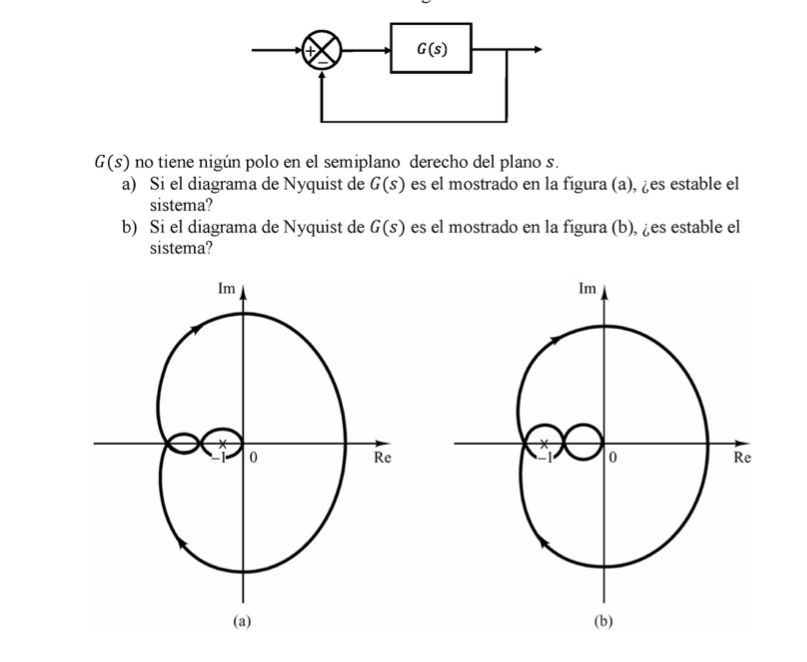
\includegraphics[width=2.5in]{imagenes/EjemploNyquist.png}
    \caption{Ejercicio [2]}
    \label{niquist-function}
    \end{figure}
\end{itemize}
\end{justify}
\end{frame}

\begin{frame}{Resumen: Estabilidad de Nyquist}
\begin{justify}
\begin{multicols}{2}
\begin{itemize}
    \item Caso 1:
    \item Tramo I:
    \\
    $s=j\omega$,
    $0\leq\omega\leq\infty$  
    \item Tramo II:
    \\
    $s=Re^{j\phi}$
    $-90^\circ\leq\phi\leq90^\circ$     
    \item Tramo III:
    \\
    Reflejo de I
\end{itemize}

\begin{itemize}
    \begin{figure}[H]
    \centering
    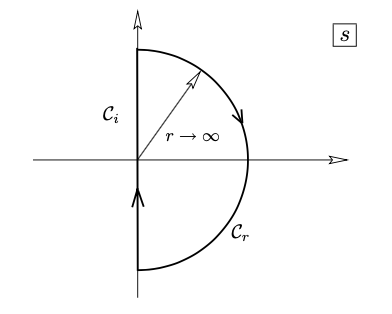
\includegraphics[width=1.5in]{imagenes/nyquist-path.png}
    \caption{Nyquist path}
    \label{niquist-function}
    \end{figure}
\end{itemize}
\end{multicols}
\end{justify}
\end{frame}

\begin{frame}{Resumen: Estabilidad de Nyquist}
\begin{justify}
\begin{multicols}{2}
\begin{itemize}
    \item Caso 2:
    \item I:
    \\
    $s=j\omega$
    \\
    $\epsilon\leq\omega\leq\infty$  
    \\
    \item II:
    \\
    $s=Re^{j\phi}$
    $R\rightarrow\infty$
    $-90^\circ\leq\phi\leq90^\circ$     
    \\
    \item III:
    Reflejo de I
    \\
    \item IV:
    \\
    $s=\epsilon e^{j\phi}$
    $\epsilon \rightarrow 0$
    $-90^\circ\leq\phi\leq90^\circ$  
\end{itemize}

\begin{itemize}
    \begin{figure}[H]
    \centering
    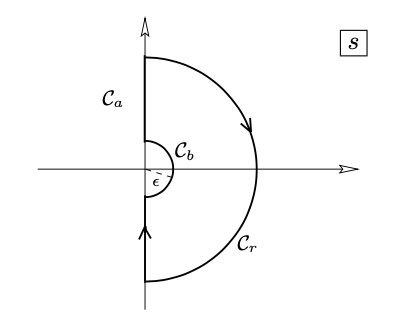
\includegraphics[width=1.5in]{imagenes/nyquist-modificado.png}
    \caption{Nyquist path con un cero en (0,0)}
    \label{niquist-function}
    \end{figure}
\end{itemize}
\end{multicols}
\end{justify}
\end{frame}

\begin{frame}{Ejemplo: Estabilidad de Nyquist}
\begin{justify}
\begin{itemize}
 \item Ejercicio [3]. Suponga que se tiene una función de transferencia en bucle abierto como:
 \begin{equation} \label{margeng1}
    FT_{ba}=\frac{K(s+2)}{(s+1)(s+3)},  Z=P+N, 
  \end{equation}
\begin{multicols}{2}
\begin{itemize}
    \\
    \item Tramo I:
    \\
    $s=j\omega$,
    \\
    $0\leq\omega\leq\infty$  
    \\  
    \item Tramo II:
    \\
    $s=Re^{j\phi}$
    \\
     $-90^\circ\leq\phi\leq90^\circ$     
    \\
    
\end{itemize}
\begin{itemize}
     \item Tramo I:
     \\
     $FT_{ba}=\frac{(j\omega+2)}{(j\omega+1)(j\omega+3)}$
     \\
     \item Tramo II:
     \\
     $FT_{ba}=\frac{(Re^{j\phi}+2)}{(Re^{j\phi}+1)(Re^{j\phi}+3)}$
    \\
    \item Tramo III:
    Reflejo de I
\end{itemize}
\end{multicols}
\end{itemize}
\end{justify}
\end{frame}

\begin{frame}{Ejemplo: Estabilidad de Nyquist}
\begin{justify}
\begin{itemize}
  \begin{figure}[H]
    \centering
    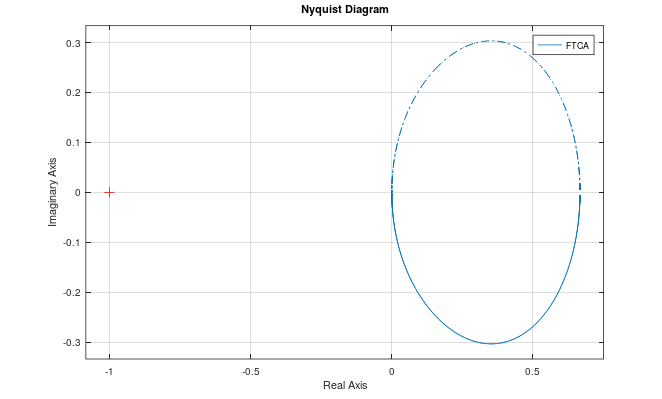
\includegraphics[width=3in]{imagenes/NyquistK1.png}
    \caption{Cuando k vale 1, el sistema es estable.}
    \label{niquist-function}
    \end{figure}
    A medida k se va haciendo menor que uno se acerca a la inestabilidad, hasta que rodea el punto -1 en el eje real.
\end{itemize}
\end{justify}
\end{frame}

\section{Estabilidad relativa: Márgenes de estabilidad y picos de sensibilidad}
\begin{frame}{Estabilidad relativa: márgenes de estabilidad y picos de sensibilidad}
\begin{justify}
\begin{itemize}
\justifying
  Suele ser deseable obtener algunas medidas cuantitativas de qué tan lejos de la inestabilidad está el bucle nominal, es decir, cuantificar la estabilidad relativa. Esto se logra introduciendo medidas que describen la distancia desde la respuesta de frecuencia nominal de bucle abierto hasta el punto crítico de estabilidad $(-1, 0)$.
  
  El margen de ganancia, $M_g$, y el margen de fase, $M_f$. Se definen de la siguiente manera:
   \begin{equation} \label{margeng1}
    M_g=-20log_{10}(\left | a \right |)
    \end{equation}
   \begin{equation} \label{margeng2}
     M_f=\phi
    \end{equation}
   
\end{itemize}
\end{justify}
\end{frame}

\begin{frame}{Estabilidad relativa: márgenes de estabilidad y picos de sensibilidad}
\begin{justify}
\begin{itemize}
  \begin{figure}[H]
    \centering
    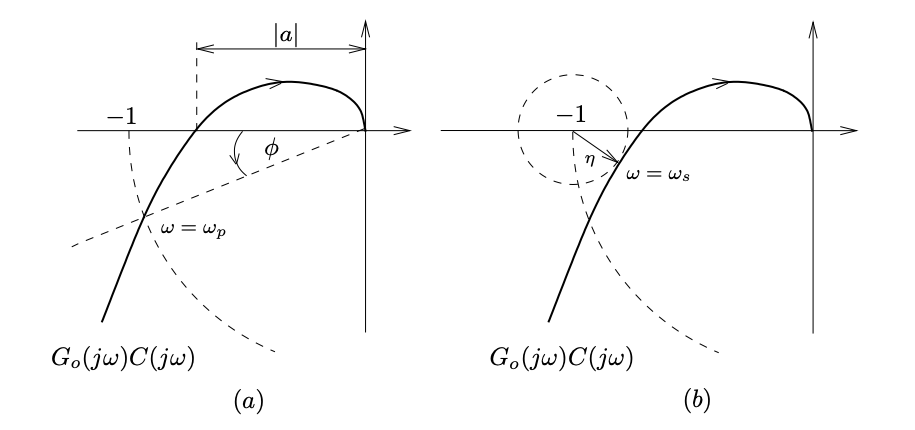
\includegraphics[width=3in]{imagenes/peak-sensibity.png}
    \caption{Márgenes de estabilidad y pico de sensibilidad.}
    \label{niquist-function}
    \end{figure}
    \item \item La parte (a) de la figura describe el margen de ganancia, $M_g$, y el margen de fase, $M_f$.
    \item La parte (b) de la figura define un indicador alternativo de estabilidad relativa.
\end{itemize}
\end{justify}
\end{frame}

\begin{frame}{Estabilidad relativa: márgenes de estabilidad y picos de sensibilidad}
\begin{justify}
\begin{itemize}
\item Los margenes de estabilidad usando diagramas de Bode
  \begin{figure}[H]
    \centering
    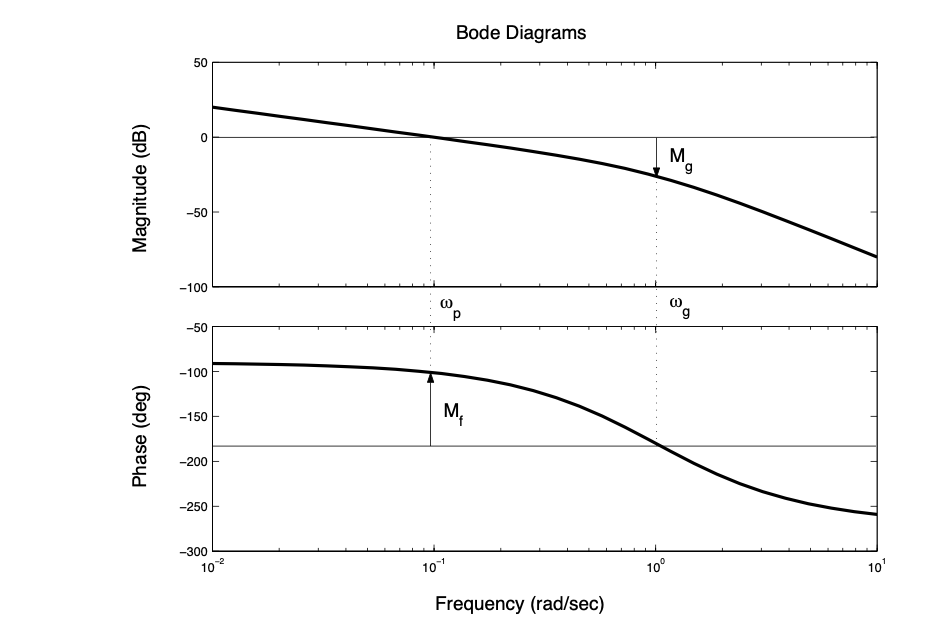
\includegraphics[width=2in]{imagenes/bode-diagram.png}
    \caption{Márgenes de estabilidad y pico de sensibilidad.}
    \label{niquist-function}
    \end{figure}
    \item La frecuencia $\omega_p$ corresponde al cual la magnitud es 0 [dB]. Esto permite calcular el Mf.
    \item La segunda frecuencia, $\omega_g$, corresponde al cual la fase es −180 grados. Esto permite calcular el Mg.
\end{itemize}
\end{justify}
\end{frame}

\section{Robustez}
\begin{frame}{Robustez}
\begin{justify}
\begin{itemize}
\justifying
 En la práctica, normalmente nos interesa no sólo el rendimiento nominal, sino también el rendimiento real logrado cuando el controlador se aplica a la planta real. Esta es la denominada cuestión de “robustez”.
\\
 Contrastamos las sensibilidades nominales derivadas anteriormente con las sensibilidades logradas (o verdaderas) cuando se aplica el controlador C(s) a algunos modelos de calibración, G(s). Queda:

\end{itemize}
\end{justify}
\end{frame}

\section{Sensibilidad alcanzada}
\begin{frame}{Sensibilidad alcanzada}
\begin{justify}
\begin{itemize}

 \begin{equation} \label{sensibilidad1}
    T(s) \stackrel{\Delta}{=} \frac{G(s)C(s)}{1+G(s)C(s)} = \frac{B(s)P(s)}{A(s)L(s) + B(s)P(s)}
\end{equation}
\begin{equation}\label{sensibilidad2}
    S(s) \stackrel{\Delta}{=} \frac{1}{1+G(s)C(s)} = \frac{A(s)L(s)}{A(s)L(s) + B(s)P(s)}
\end{equation}
\begin{equation}\label{sensibilidad3}
    S_{i} (s) \stackrel{\Delta}{=} \frac{G(s)}{1+G(s)C(s)} = \frac{B(s)L(s)}{A(s)L(s) + B(s)P(s)}
\end{equation}
\begin{equation}\label{sensibilidad4}
    S_{u} (s) \stackrel{\Delta}{=} \frac{C(s)}{1+G(s)C(s)} = \frac{A(s)P(s)}{A(s)L(s) + B(s)P(s)}
\end{equation}
\end{itemize}
\end{justify}
\end{frame}

\section{Estabilidad Robusta}
\begin{frame}{Estabilidad Robusta}
\begin{justify}
\begin{itemize}
\justifying
 Nos preocupa el caso en el que el modelo nominal y la planta real difieren. Entonces es necesario que, además de la estabilidad nominal, comprobemos que la estabilidad se mantiene cuando la verdadera planta está controlada por el mismo controlador. A esta propiedad la llamamos estabilidad robusta.
Las condiciones suficientes para que un circuito de retroalimentación sea sólidamente estable se establecen a continuación:

\end{itemize}
\end{justify}
\end{frame}

\begin{frame}{Estabilidad Robusta}
\begin{justify}

\begin{itemize}
\justifying
 Teorema de estabilidad robusta: Considere una planta con función de transferencia nominal $G_o(s)$ y función de transferencia verdadera dada por G(s). Supongamos que C(s) es la función de transferencia de un controlador que logra estabilidad interna nominal. Supongamos también que G(s)C(s) y Go(s)C(s) tienen el mismo número de polos inestables. Entonces, una condición suficiente para la estabilidad del circuito de retroalimentación verdadero obtenido al aplicar el controlador a la planta verdadera es que

 \begin{equation}\label{sensibilidad3}
    \left |{ T_{o } (j\omega)}  \right | \left |{ G_{\Delta } (j\omega)}  \right |=\left |\frac{G_o(j\omega)C(j\omega)}{1+G_o(j\omega)C(j\omega)}  \right | \left |{ G_{\Delta } (j\omega)}  \right |<1
\end{equation}
\end{itemize}

\end{justify}
\end{frame}

\begin{frame}{Estabilidad Robusta}
\begin{justify}
\begin{itemize}
\begin{figure}[H]
    \centering
    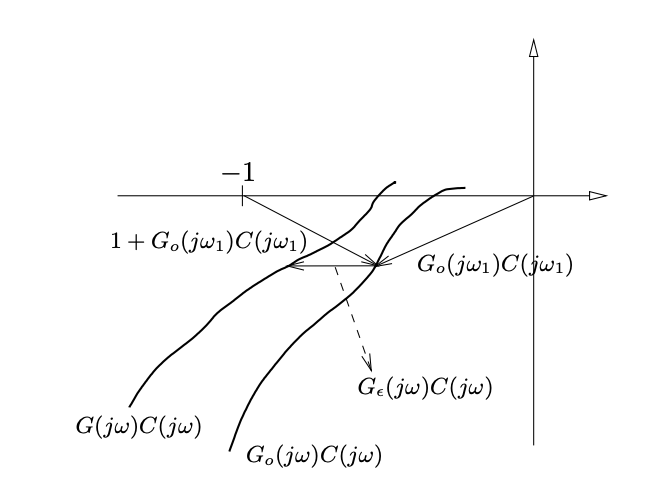
\includegraphics[width=2.5in]{imagenes/nyquist-nominal-true.png}
    \caption{Gráfico de Nyquist para el bucle nominal y verdadero}
    \label{niquist-function}
    \end{figure}
\end{itemize}
\end{justify}
\end{frame}

\begin{frame}{Estabilidad Robusta}
\begin{justify}

\begin{itemize}
\justifying
Primero recordamos que, por supuesto, el bucle nominal es estable y que $G(s)C(s)$ y $G_o(s)C(s)$ tienen el mismo número de polos inestables.
\\
Esto significa que el bucle real será estable si y sólo si el gráfico de Nyquist de $G(j\omega)C(j\omega)$ rodea el punto $(−1, 0)$ el mismo número de veces (y en la misma dirección) que $G_o(j\omega)C(j\omega)$.
\\
También tenemos que:
 \begin{equation}\label{sensibilidad3}
   G(s)C(s)=G_o(s)C(s)+G_\epsilon (s)C(s)
\end{equation}
Es decir, el cambio en la función de transferencia de bucle abierto es $G_{\epsilon}(s)C(s)$, donde $G_{\epsilon}(s)C(s)$ es la respuesta de frecuencia del error de modelado aditivo (AME).
\end{itemize}
\end{justify}
\end{frame}

\begin{frame}{Estabilidad Robusta}
\begin{justify}
\begin{itemize}
\justifying
De esa figura vemos que ocurre el mismo número de vueltas si:
\begin{equation}\label{sensibilidad3}
   \left |{ G{\epsilon}(j\omega)C(j\omega)}  \right |< \left |{ 1+ G_{o}(j\omega)C(j\omega)}  \right |
\end{equation}
Recalcando que $G_{\epsilon}(s)=C(s)G_{\Delta}(s)$ y notando que la ecuación anterior es equivalente a:
\begin{equation}\label{sensibilidad3}
   \frac{\left |{ G_{\Delta}(j\omega)G(j\omega)C(j\omega)}  \right |}{\left |{ 1+G{o}(j\omega)C(j\omega)}  \right |}<1 
\end{equation}
\\
Esta es la misma que la que definimos en el teorema de control robusto.
\end{itemize}
\end{justify}
\end{frame}

\begin{frame}{Estabilidad Robusta}
\begin{justify}
\begin{itemize}
\justifying
\item Observación 1: El teorema proporciona sólo una condición suficiente para una estabilidad robusta.
\item Observación 2: El teorema  también se aplica a sistemas de tiempo discreto y de datos muestreados, siempre que se utilice la función de respuesta de frecuencia adecuada.
\item Observación 3: También es posible extender el teorema al caso en que  $G_{\Delta }(s)$ es inestable.
\item Observación 4: Al aplicar el resultado de estabilidad robusta es habitual que $\left |G_{\Delta }(j\omega) \right |$ se reemplaza por algún límite superior conocido, digamos $\epsilon$($\omega$). La condición suficiente puede entonces sustituirse por $\left |T_{o}(j\omega)\epsilon(j\omega) \right |<1, \forall \omega$
\end{itemize}
\end{justify}
\end{frame}

\begin{frame}{Ejemplo: Estabilidad Robusta}
\begin{justify}
\begin{itemize}
\justifying
\item En un bucle de control de retroalimentación, la función de transferencia de bucle abierto está dada por:
 \begin{equation}\label{robustez1}
   G_o(s)C(s) = \frac{0.5}{s(s+1)^2}   
\end{equation}
\item Y la funcion de transferencia de la parte real es:
 \begin{equation}\label{robustez2}
    G(s) = e^{-s\tau}G_o(s)   
\end{equation}
\item Encuentre el valor exacto de $\tau$ que lleva el circuito cerrado al borde de la inestabilidad.
\item Utilice el teorema de estabilidad robusta para obtener una estimación de ese valor crítico de $\tau$.
\item Discuta por qué los resultados anteriores difieren.
\end{itemize}
\end{justify}
\end{frame}

\begin{frame}{Solución: Estabilidad Robusta}
\begin{justify}
\begin{itemize}
\justifying
\item El retraso introduce un cambio de fase igual a $-\omega \tau$. Por lo tanto, la condición crítica de estabilidad surge cuando este retraso es igual al margen de fase:
 \begin{equation}\label{robustez3}
    \tau = \frac{M_f}{\omega_p}=\frac{0.77[rad]}{0.424[rad/s] }  =1.816s 
\end{equation}
\item La sensibilidad complementaria nominal viene dada por
 \begin{equation}\label{robustez4}
    T_o(s) = \frac{G_o(s)C(s)}{1+G_o(s)C(s)}=\frac{0.5}{s^3+2s^2+s+0.5}
\end{equation}

\end{itemize}
\end{justify}
\end{frame}

\begin{frame}{Solución: Estabilidad Robusta}
\begin{justify}
\begin{itemize}
\justifying
\item Y el error de modelado multiplicativo es:
 \begin{equation}\label{robustez3}
    G_{\Delta}(s) = \frac{G(s)-G_o(s)}{G_o(s)}=\frac{e^{-s\tau}G_o(s)-G_o(s)}{G_o(s)}=e^{-s\tau}-1
\end{equation}
\item La magnitud viene dada por:
 \begin{equation}\label{robustez4}
    \left |G_{\Delta}(j\omega)\right| =  \left |sen(\omega\tau/2)\right|
\end{equation}
\item Entonces tenemos que:
 \begin{equation}\label{robustez4}
    \left |T_o(s)G_{\Delta}(j\omega)\right| =  \left |sen(\omega\tau/2)\right| \left |\frac{0.5}{(j\omega)^3+2(j\omega)^2+(j\omega)+0.5}\right| < 1
\end{equation}
\end{itemize}
\end{justify}
\end{frame}

\begin{frame}{Solución: Estabilidad Robusta}
\begin{justify}
\begin{itemize}
\justifying
\item Se probaron varios valores de $\tau$. Algunos de estos resultados se muestran a continuación:
\centering
\begin{figure}
    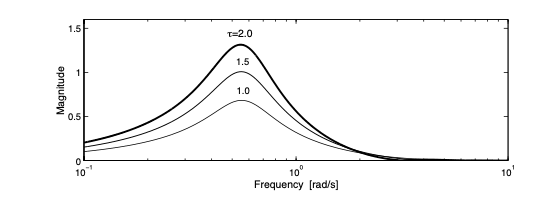
\includegraphics[width=3in]{imagenes/estabilidadRobustaEjemplo.png}
    \caption{Magnitud de la respuesta en frecuencia de $T_o(s)G_{\Delta}(s)$ para diferentes valores de $\tau$}
    \label{niquist-function}
\end{figure}
\item Se concluye que el valor de  $\tau$ debe ser de 1.5 para que la cota sea $<$ 1.   
\end{itemize}
\end{justify}
\end{frame}

\begin{frame}{Referencias}
\begin{justify}
\begin{itemize}
\justifying
[1] Christian Trejo, Sistemas Dinámicos y Control, «Ejercicio Lugar geométrico de las raíces, ángulos, asíntotas, centroide, ruptura y ganancia», YouTube. 1 de noviembre de 2022. [En línea]. Disponible en: https://www.youtube.com/watch?v=XSMLFjYFud0
\break
[2] UNI NOW ACADEMIA, «Criterio Nyquist Estabilidad #Nyquist Camino y diagrama estabilidad», YouTube. 1 de noviembre de 2020. [En línea]. Disponible en: https://www.youtube.com/watch?v=2cu1RGbyGNs
\break
[3] UNI NOW ACADEMIA, «Nyquist tipo 1, compruebo la estabilidad para todos los valores de K», YouTube. 7 de diciembre de 2020. [En línea]. Disponible en: https://www.youtube.com/watch?v=cqHNKr1IM30
\end{itemize}
\end{justify}
\end{frame}
 \end{document}